\documentclass[11pt]{article}
\usepackage[margin=22mm]{geometry}
\usepackage{newtxtext,newtxmath,graphicx,booktabs,float,hyperref,listings,xcolor}
\hypersetup{colorlinks=true,urlcolor=blue,linkcolor=blue}
\lstset{basicstyle=\ttfamily\scriptsize,breaklines=true,numbers=left,numberstyle=\tiny,frame=single}
\title{Iris Phenolic Liners\\Continuous-Heating Campaign}
\author{MIT Rocket Team --- exploratory numerical study}
\date{November 05, 2026, 20:05 EST}
\begin{document}\maketitle
\begin{center}\textbf{Setup and provisional numerical diagnostics.\\No validated motor burnthrough time is claimed.}\end{center}
\section{New objective and current execution}
The November 5 instruction is to choose the exposure duration and answer when
the liner is exhausted, rather than repeatedly demonstrating seven-second
survival. Four fresh independent radial calculations therefore apply continuous
nominal heating until the finite-row model records exhaustion. They are not
native ANSYS results. The already-running CF320 ANSYS verification remains
intact on ten SMP cores; subsequent short-pulse jobs have been deferred.

The environment retains gas temperature 2504 K (2230.85 C), uncorrected
convection coefficient 1000 W/(m$^2$ K), nominal chamber pressure 800 psi,
the documented blowing correction and zero effective hot-side radiation.
Initial liner thickness is 4.7625 mm for the sustainer and 6.3500 mm for the
booster. These scouts use 160 liner and 40 casing cells and a 0.0015625 s step
ceiling. Reporting milestones extend from 30 to 960 s without switching off
heating at seven seconds. The chosen environment is hypothetical, not an
inferred propellant burn duration.

\section{First continuous-heating outcomes}
\begin{table}[H]\centering
\begin{tabular}{lrr}\toprule
Case & Model exhaustion [s] & Earlier property flag [s]\\\midrule
Sustainer Al & 114.9 & 49.6 \\
Sustainer CF & 112.2 & 18.5 \\
Booster Al & 151.7 & 87.4 \\
Booster CF & 147.0 & 32.9 \\
\bottomrule\end{tabular}
\caption{Coarse numerical events of the inherited finite-row closure. All occur
after the casing model has left its provisional property range. These are
not accepted physical motor lifetimes or allowable firing durations.}
\end{table}
The arithmetic now reaches the requested geometric endpoint. It does not yet
establish its credibility: neither time/mesh convergence of these events nor
high-temperature casing validity has been demonstrated. The prior rejected
endurance calculations remain rejected and are not the source of this table.
The first 150 C CF or 300 C Al property-range crossing is recorded separately;
these are evidence-range flags, not certified structural failure temperatures.
Beyond them the equations continue with the inherited surrogate properties.

Source/configuration fingerprints, checkpoint continuity, final-row bookkeeping,
monotone sampled time and the cumulative mass ledger pass. Maximum cumulative
mass relative error is 1.54e-14, and maximum step equation-energy residual is
4.2e-11. Closing that discrete energy equation does not prove a physically
complete open-system enthalpy model. Every record retains
\texttt{eligible\_for\_motor\_lifetime=false}.

\begin{figure}[H]\centering
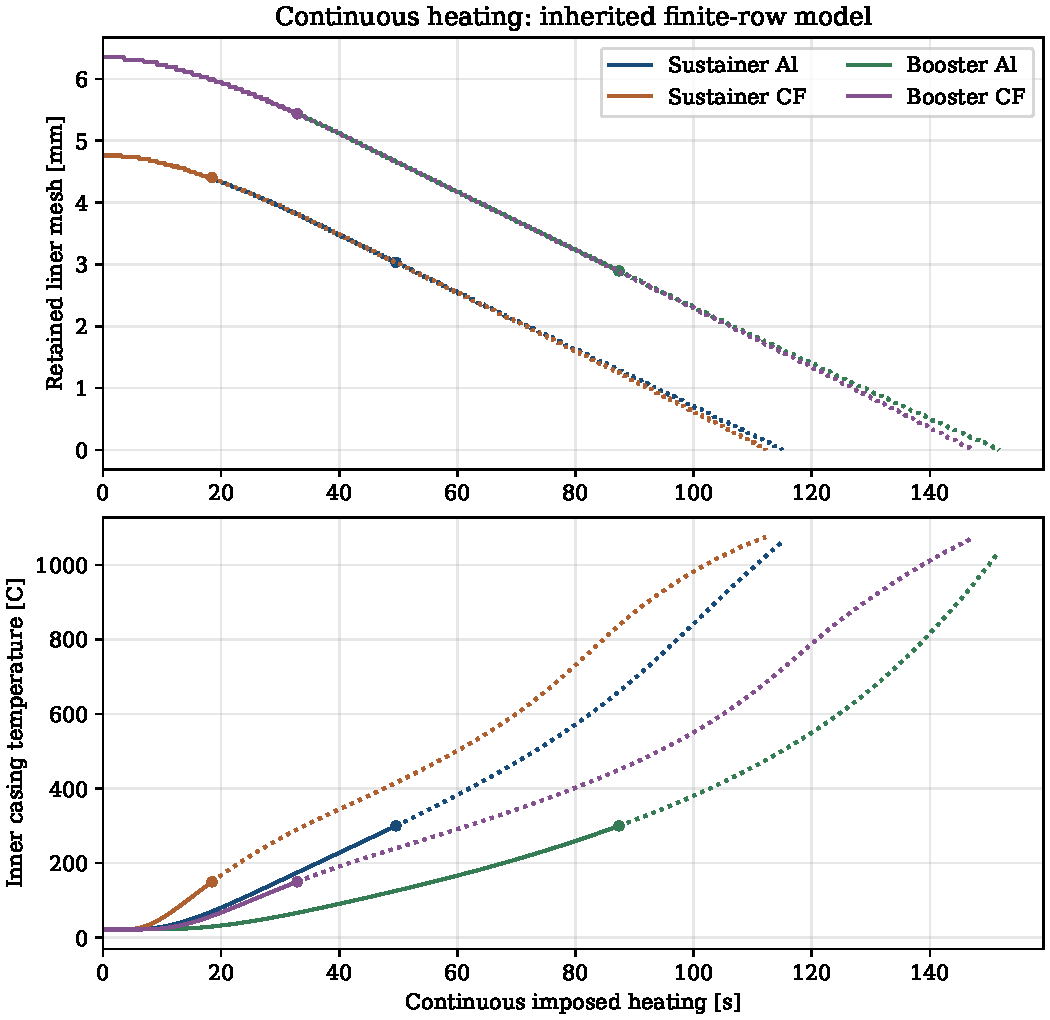
\includegraphics[width=\textwidth]{../analysis/continuous_heating_scouts.pdf}
\caption{Independent mathematical scouts. Dots mark the first casing-property
flag; dotted curves are subsequent surrogate continuation. Remaining thickness
is retained mesh, including char, not the thickness of undamaged virgin resin.}
\end{figure}

\section{Numerical checks now prepared}
For each motor, a 160/40-cell calculation at half the step isolates temporal
error. A subsequent 320/80-cell calculation at that same smaller step isolates
spatial change. Those eight calculations are separate from the four scouts;
their preparation is not a convergence result. Further 640-cell and time checks
follow where required. Event-time change must be below five percent, with
intermediate retained-thickness agreement within the larger of 0.02 mm or one
percent of initial thickness. Surface histories need their own assessment.

\section{Model improvements and implemented first component}
The priority is a conservative moving surface. In the old model, partially
consumed rows retain thermal capacity until a residual-mass threshold removes
them. This couples the apparent recession to row width and cutoff. The new
candidate will update occupied volume, conductive paths and stored enthalpy
as the surface moves. The surface velocity must follow a mass/energy closure
that distinguishes unreacted material, char and escaping gas.

The geometry/remapping component is implemented and tested separately. In the
cylindrical volume coordinate $x=r^2/2$, each conserved field $u$ satisfies
\[
 I_i=\int_{r_i}^{r_{i+1}}u(r)r\,dr,\qquad
 \sum I_{\rm old}=\sum I_{\rm retained}+I_{\rm swept}.
\]
It remaps extensive mass and enthalpy, not temperature and conversion
independently, and returns swept-out quantities explicitly. Analytic nonuniform
overlap, zero-motion and prescribed pure-char front tests pass at three
resolutions. The artificial 100 s front benchmark is a verification input,
not an Iris result. No cell or heat capacity remains after exact domain exhaustion.

\textbf{This component is not yet a coupled thermal/pyrolysis solver.}
Next implement thermodynamic reconstruction, reaction/gas enthalpy terms,
conservative front transport and an iterated surface energy balance without
double-counting removal energy. Then verify a Stefan-type moving-front limit,
reaction limits and integrated mass/energy before native adoption. New ANSYS
packages will preserve the original sealed runs and restart lineage.

High-temperature Al properties/phase change and CF resin decomposition need
documented surrogates; otherwise post-range results remain conditional intact-
backing scenarios. Heat-transfer, radiation and char-consumption sensitivities
must accompany any eventual event-time range. Measured liner recession and
actual exposure history remain the strongest missing physical constraints.

Moving-grid energy, decomposition and surface balances are established elements
of charring-ablation modelling; see Chen and Milos (2013),
\href{https://ntrs.nasa.gov/citations/20130014432}{NASA NTRS 20130014432}.
Its PICA/re-entry parameters are not calibration data for this motor.

\appendix\section{Candidate conservative geometry kernel}
Complete source below. This is a new independent component; the earlier full
MAPDL/Fortran listings remain in the main report. No native thermal law has
been replaced by this kernel yet.
\lstinputlisting[language=Python]{../../model/moving_surface_remap.py}
\end{document}
